\documentclass[%
  crop,%
  tikz,%
  multi=false%
]{standalone}%
\usepackage[utf8]{luainputenc}%
\usepackage[no-math]{fontspec}%
\defaultfontfeatures{%
  Numbers={OldStyle,Proportional},%
  Ligatures=TeX,%
  Extension=.ttf,%
}%
\setmainfont[%
  UprightFont=*-Regular,%
  ItalicFont=*-Italic,%
  BoldFont=*-Bold,%
  BoldItalicFont=*-BoldItalic,%
]{Raleway}%
\setsansfont[%
  UprightFont=*-Regular,%
  ItalicFont=*-Italic,%
  BoldFont=*-Bold,%
  BoldItalicFont=*-BoldItalic,%
]{Raleway}%
\usepackage[frenchmath]{mathastext}%
\usepackage{amsmath}%
\usepackage{amssymb}%
\usepackage{mathrsfs}%
\usepackage{mathtools}%
\usepackage{siunitx}%
\usepackage[siunitx]{circuitikz}%
\usetikzlibrary{calc,backgrounds,arrows.meta,patterns,positioning}%
\ctikzset{bipoles/length=1.2cm}%

% Colors
\usepackage{xcolor}%
\definecolor{RoseauGreen}{HTML}{cad40e}%
\definecolor{RoseauGrey}{HTML}{adb9cb}%
\definecolor{RoseauBlue}{HTML}{234e83}%

\DeclareMathOperator{\sign}{sign}%

% Sets
\let\C\relax
\newcommand{\R}{\ensuremath{\mathbb{R}}} % Real
\newcommand{\N}{\ensuremath{\mathbb{N}}} % Natural
% \newcommand{\C}{\ensuremath{\mathbb{C}}} % Complexes
\newcommand{\B}{\ensuremath{\mathscr{B}}} % Electrical buses
\newcommand{\Ch}{\ensuremath{\mathscr{C}}} % Loads
\renewcommand{\L}{\ensuremath{\mathscr{L}}} % Lines
\renewcommand{\P}{\ensuremath{\mathscr{P}}} % Phases

% Phases
\newcommand{\arm}{\ensuremath{\mathrm{a}}}%
\newcommand{\brm}{\ensuremath{\mathrm{b}}}%
\newcommand{\crm}{\ensuremath{\mathrm{c}}}%
\newcommand{\nrm}{\ensuremath{\mathrm{n}}}%
\newcommand{\grm}{\ensuremath{\mathrm{g}}}%
\newcommand{\abrm}{\ensuremath{\mathrm{ab}}}%
\newcommand{\bcrm}{\ensuremath{\mathrm{bc}}}%
\newcommand{\carm}{\ensuremath{\mathrm{ca}}}%
\newcommand{\anrm}{\ensuremath{\mathrm{an}}}%
\newcommand{\bnrm}{\ensuremath{\mathrm{bn}}}%
\newcommand{\cnrm}{\ensuremath{\mathrm{cn}}}%
\newcommand{\agrm}{\ensuremath{\mathrm{ag}}}%
\newcommand{\bgrm}{\ensuremath{\mathrm{bg}}}%
\newcommand{\cgrm}{\ensuremath{\mathrm{cg}}}%
\newcommand{\ngrm}{\ensuremath{\mathrm{ng}}}%
\newcommand{\abcrm}{\ensuremath{\mathrm{abc}}}%
\newcommand{\abcnrm}{\ensuremath{\mathrm{abcn}}}%

% Transformer
\newcommand{\Xrm}{\ensuremath{\mathrm{X}}}%
\newcommand{\Yrm}{\ensuremath{\mathrm{Y}}}%
\newcommand{\Zrm}{\ensuremath{\mathrm{Z}}}%
\newcommand{\xrm}{\ensuremath{\mathrm{x}}}%
\newcommand{\yrm}{\ensuremath{\mathrm{y}}}%
\newcommand{\zrm}{\ensuremath{\mathrm{z}}}%
\newcommand{\Arm}{\ensuremath{\mathrm{A}}}%
\newcommand{\Brm}{\ensuremath{\mathrm{B}}}%
\newcommand{\Crm}{\ensuremath{\mathrm{C}}}%
\newcommand{\Nrm}{\ensuremath{\mathrm{N}}}%

% Indices or exponents
\newcommand{\cons}{\ensuremath{\mathrm{cons.}}}%
\renewcommand{\prod}{\ensuremath{\mathrm{prod.}}}%
\newcommand{\theo}{\ensuremath{\mathrm{th.}}}%
\newcommand{\const}{\ensuremath{\mathrm{const.}}}%

% Variables
\newcommand{\umax}{\ensuremath{U^{\max}}}%
\newcommand{\umaxnorm}{\ensuremath{U^{\max\,\text{norm.}}}}%
\newcommand{\umin}{\ensuremath{U^{\min}}}%
\newcommand{\uminnorm}{\ensuremath{U^{\min\,\text{norm.}}}}%
\newcommand{\unom}{\ensuremath{U^{\text{nom.}}}}%
\newcommand{\unomnorm}{\ensuremath{U^{\text{nom.}\,\text{norm.}}}}%
\newcommand{\uup}{\ensuremath{U^{\text{up}}}}%
\newcommand{\uupnorm}{\ensuremath{U^{\text{up}\,\text{norm.}}}}%
\newcommand{\uupprime}{\ensuremath{U^{\text{up}\,\prime}}}%
\newcommand{\udown}{\ensuremath{U^{\text{down}}}}%
\newcommand{\udownnorm}{\ensuremath{U^{\text{down}\,\text{norm.}}}}%
\newcommand{\udownprime}{\ensuremath{U^{\text{down}\,\prime}}}%
\newcommand{\smax}{\ensuremath{S^{\max}}}%
\newcommand{\pmax}{\ensuremath{P^{\max}}}%
\newcommand{\sproj}{\ensuremath{\underline{S^{\text{proj.}}}}}%
%

\begin{document}
\ctikzset{european, straight voltages, cute inductors, bipoles/length=1cm, voltage shift=0.5mm}%
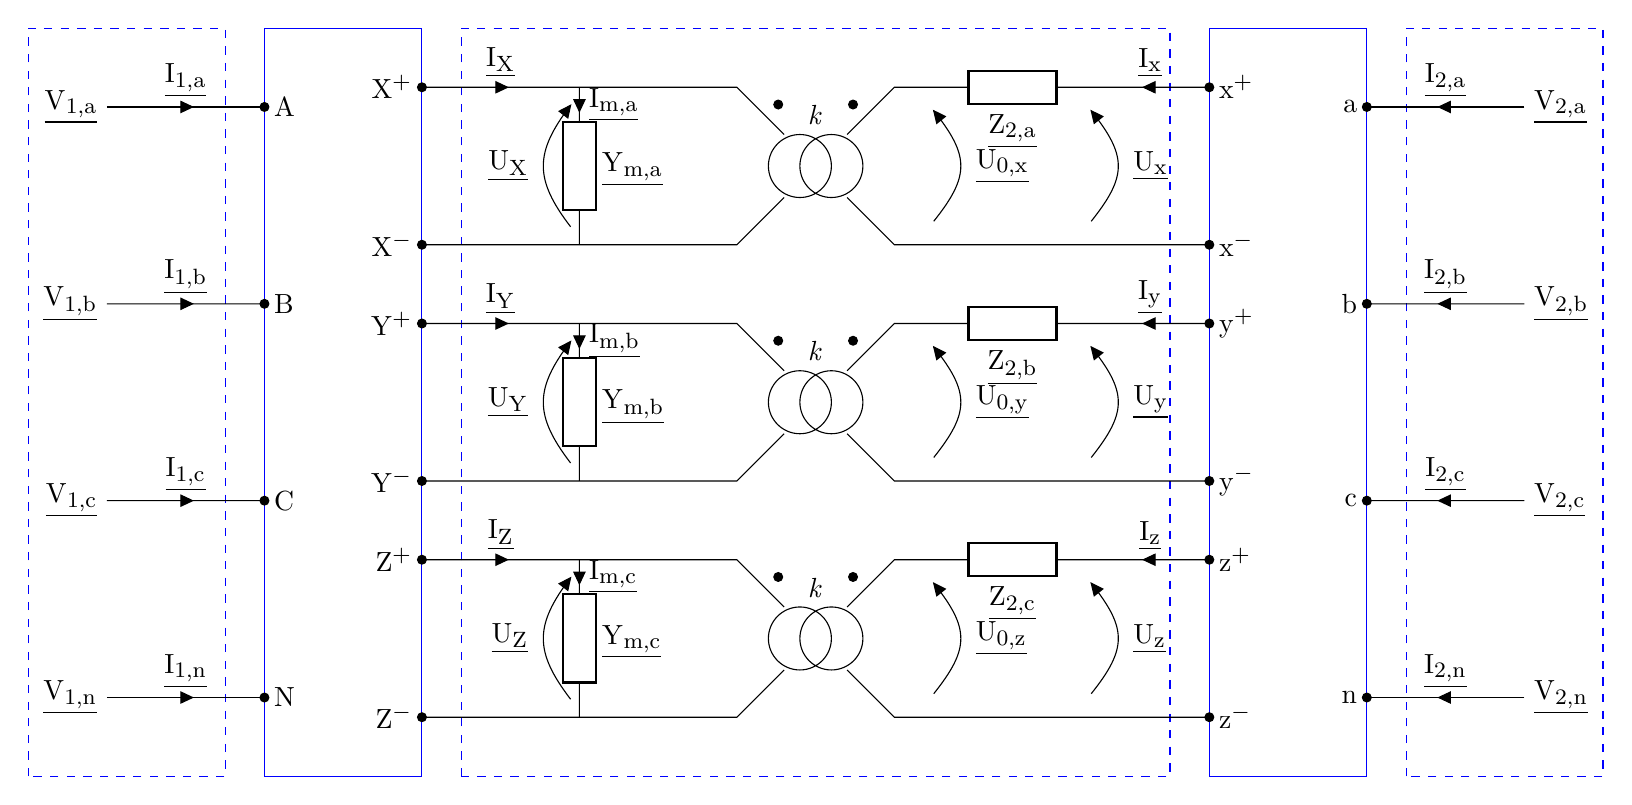
\begin{tikzpicture}[%
    show background rectangle,%
    tight background,%
    background rectangle/.style={fill=white}%
  ]
  %
  % Définitions
  %
  % No European transformer in circuitikz [BV, 17/07/2023]
  \tikzset{
    transformer/.pic={
      \draw (-0.2,0) circle[radius=0.4] (0.2,0) circle[radius=0.4];
    },
  }
  \pgfmathsetmacro{\xzero}{0};%
  \pgfmathsetmacro{\xone}{1};%
  \pgfmathsetmacro{\xtwo}{3};%
  \pgfmathsetmacro{\xthree}{5};%
  \pgfmathsetmacro{\xym}{7};%
  \pgfmathsetmacro{\xtransformer}{10};%
  \pgfmathsetmacro{\xtransformerm}{\xtransformer-1};%
  \pgfmathsetmacro{\xtransformerp}{\xtransformer+1};%
  \pgfmathsetmacro{\xztwom}{11.5};%
  \pgfmathsetmacro{\xztwop}{13.5};%
  \pgfmathsetmacro{\xfour}{15};%
  \pgfmathsetmacro{\xfive}{17};%
  \pgfmathsetmacro{\xsix}{19};%
  \pgfmathsetmacro{\xseven}{20};%
  \pgfmathsetmacro{\yn}{0};%
  \pgfmathsetmacro{\yc}{2.5};%
  \pgfmathsetmacro{\yb}{5};%
  \pgfmathsetmacro{\ya}{7.5};%
  \pgfmathsetmacro{\yxp}{\ya+0.25};%
  \pgfmathsetmacro{\yxm}{\yxp-2};%
  \pgfmathsetmacro{\yyp}{\yxm-1};%
  \pgfmathsetmacro{\yym}{\yyp-2};%
  \pgfmathsetmacro{\yzp}{\yym-1};%
  \pgfmathsetmacro{\yzm}{\yzp-2};%
  \pgfmathsetmacro{\yzero}{\yn-1};%
  \pgfmathsetmacro{\yone}{\ya+1};%

  % Rectangles
  \pgfmathsetmacro{\xtmp}{\xone+0.75*(\xtwo-\xone)};%
  \draw[blue,dashed] (\xzero, \yzero) rectangle (\xtmp,\yone);%
  \draw[blue] (\xtwo,\yzero) rectangle (\xthree,\yone);%
  \draw[blue] (\xfour, \yzero) rectangle (\xfive,\yone);%
  \pgfmathsetmacro{\xtmp}{\xsix-0.75*(\xsix-\xfive)};%
  \draw[blue,dashed] (\xtmp, \yzero) rectangle (\xseven,\yone);%

  \pgfmathsetmacro{\xtmpleft}{\xthree+0.5};%
  \pgfmathsetmacro{\xtmpright}{\xfour-0.5};%
  \draw[blue,dashed] (\xtmpleft, \yzero) rectangle (\xtmpright,\yone);%

  % ABCN
  \draw (\xone,\ya) node[left] {$\underline{V_{1,\arm}}$}%
  to[short,-*,i=$\underline{I_{1,\arm}}$] (\xtwo,\ya) node[right] {$\Arm$};%
  \draw (\xone,\yb) node[left] {$\underline{V_{1,\brm}}$}%
  to[short,-*,i=$\underline{I_{1,\brm}}$] (\xtwo,\yb) node[right] {$\Brm$};%
  \draw (\xone,\yc) node[left] {$\underline{V_{1,\crm}}$}%
  to[short,-*,i=$\underline{I_{1,\crm}}$] (\xtwo,\yc) node[right] {$\Crm$};%
  \draw (\xone,\yn) node[left] {$\underline{V_{1,\nrm}}$}%
  to[short,-*,i=$\underline{I_{1,\nrm}}$] (\xtwo,\yn) node[right] {$\Nrm$};%

  % XYZ
  % First winding (X)
  \pgfmathsetmacro{\ytmp}{0.5*(\yxp+\yxm)};%
  \pic[local bounding box=TX] at (\xtransformer,\ytmp) {transformer};%
  \draw (\xthree,\yxp) node[left] {$\Xrm^+$}%
  to[short,*-,i=$\underline{I_{\Xrm}}$] (\xym,\yxp)%
  to[short] (\xtransformerm,\yxp)%
  to[short] node[near start,above=0.25cm,circ] {} (TX);%
  \draw (\xthree,\yxm) node[left] {$\Xrm^-$}%
  to[short,*-] (\xym,\yxm)%
  to[short] (\xtransformerm,\yxm)%
  to[short] (TX);%
  \draw (\xym,\yxp) to[generic,%
    i>^=$\underline{I_{\mathrm{m},\arm}}$,%
    l=$\underline{Y_{\mathrm{m},\arm}}$,%
    v<=$\underline{U_{\Xrm}}$%
  ] (\xym,\yxm);%
  \node[above] at (TX.north) {$k$};%

  % First winding (Y)
  \pgfmathsetmacro{\ytmp}{0.5*(\yyp+\yym)};%
  \pic[local bounding box=TY] at (\xtransformer,\ytmp) {transformer};%
  \draw (\xthree,\yyp) node[left] {$\Yrm^+$}%
  to[short,*-,i=$\underline{I_{\Yrm}}$] (\xym,\yyp)%
  to[short] (\xtransformerm,\yyp)%
  to[short] node[near start,above=0.25cm,circ] {} (TY);%
  \draw (\xthree,\yym) node[left] {$\Yrm^-$}%
  to[short,*-] (\xym,\yym)%
  to[short] (\xtransformerm,\yym)%
  to[short] (TY);%
  \draw (\xym,\yyp) to[generic,%
    i>^=$\underline{I_{\mathrm{m},\brm}}$,%
    l=$\underline{Y_{\mathrm{m},\brm}}$,%
    v<=$\underline{U_{\Yrm}}$%
  ] (\xym,\yym);%
  \node[above] at (TY.north) {$k$};%

  % First winding (Z)
  \pgfmathsetmacro{\ytmp}{0.5*(\yzp+\yzm)};%
  \pic[local bounding box=TZ] at (\xtransformer,\ytmp) {transformer};%
  \draw (\xthree,\yzp) node[left] {$\Zrm^+$}%
  to[short,*-,i=$\underline{I_{\Zrm}}$] (\xym,\yzp)%
  to[short] (\xtransformerm,\yzp)%
  to[short] node[near start,above=0.25cm,circ] {} (TZ);%
  \draw (\xthree,\yzm) node[left] {$\Zrm^-$}%
  to[short,*-] (\xym,\yzm)%
  to[short] (\xtransformerm,\yzm)%
  to[short] (TZ);%
  \draw (\xym,\yzp) to[generic,%
    i>^=$\underline{I_{\mathrm{m},\crm}}$,%
    l=$\underline{Y_{\mathrm{m},\crm}}$,%
    v<=$\underline{U_{\Zrm}}$%
  ] (\xym,\yzm);%
  \node[above] at (TZ.north) {$k$};%

  % xyz
  % Second winding (x)
  \pgfmathsetmacro{\ytmp}{0.5*(\yxp+\yxm)};%
  \draw (\xfour,\yxp) node[right] {$\xrm^+$}%
  to[short,*-,i>_=$\underline{I_{\xrm}}$] (\xztwop, \yxp)%
  to[generic,l=$\underline{Z_{2,\arm}}$] (\xztwom, \yxp)%
  to[short] (\xtransformerp,\yxp) %
  to[short] node[near start,above=0.25cm,circ] {} (TX);%
  \draw (\xfour,\yxm) node[right] {$\xrm^-$}%
  to[short,*-] (\xtransformerp,\yxm) to[short] (TX);%
  \draw (\xztwop, \yxm) to[open,v=$\underline{U_{\xrm}}$] (\xztwop, \yxp);%
  \draw (\xztwom, \yxm) to[open,v=$\underline{U_{0,\xrm}}$] (\xztwom, \yxp);%

  % Second winding (y)
  \pgfmathsetmacro{\ytmp}{0.5*(\yyp+\yym)};%
  \draw (\xfour,\yyp) node[right] {$\yrm^+$}%
  to[short,*-,i>_=$\underline{I_{\yrm}}$] (\xztwop, \yyp)%
  to[generic,l=$\underline{Z_{2,\brm}}$] (\xztwom, \yyp)%
  to[short] (\xtransformerp,\yyp)%
  to[short] node[near start,above=0.25cm,circ] {} (TY);%
  \draw (\xfour,\yym) node[right] {$\yrm^-$}%
  to[short,*-] (\xtransformerp,\yym) to[short] (TY);%
  \draw (\xztwop, \yym) to[open,v=$\underline{U_{\yrm}}$] (\xztwop, \yyp);%
  \draw (\xztwom, \yym) to[open,v=$\underline{U_{0,\yrm}}$] (\xztwom, \yyp);%

  % Second winding (z)
  \pgfmathsetmacro{\ytmp}{0.5*(\yzp+\yzm)};%
  \draw (\xfour,\yzp) node[right] {$\zrm^+$}%
  to[short,*-,i>_=$\underline{I_{\zrm}}$]  (\xztwop, \yzp)%
  to[generic,l=$\underline{Z_{2,\crm}}$] (\xztwom, \yzp)%
  to[short] (\xtransformerp,\yzp)%
  to[short] node[near start,above=0.25cm,circ] {} (TZ);%
  \draw (\xfour,\yzm) node[right] {$\zrm^-$}%
  to[short,*-] (\xtransformerp,\yzm) to[short] (TZ);%
  \draw (\xztwop, \yzm) to[open,v=$\underline{U_{\zrm}}$] (\xztwop, \yzp);%
  \draw (\xztwom, \yzm) to[open,v=$\underline{U_{0,\zrm}}$] (\xztwom, \yzp);%

  % abcn
  \draw (\xsix,\ya) node[right] {$\underline{V_{2,\arm}}$}%
  to[short,-*,i_=$\underline{I_{2,\arm}}$] (\xfive,\ya) node[left] {$\arm$};%
  \draw (\xsix,\yb) node[right] {$\underline{V_{2,\brm}}$}%
  to[short,-*,i_=$\underline{I_{2,\brm}}$] (\xfive,\yb) node[left] {$\brm$};%
  \draw (\xsix,\yc) node[right] {$\underline{V_{2,\crm}}$}%
  to[short,-*,i_=$\underline{I_{2,\crm}}$] (\xfive,\yc) node[left] {$\crm$};%
  \draw (\xsix,\yn) node[right] {$\underline{V_{2,\nrm}}$}%
  to[short,-*,i_=$\underline{I_{2,\nrm}}$] (\xfive,\yn) node[left] {$\nrm$};%
\end{tikzpicture}
\end{document}
% Local Variables:
% mode: latex
% TeX-engine: luatex
% TeX-source-correlate-method-active: synctex
% ispell-local-dictionary: "british"
% coding: utf-8
% LaTeX-indent-level: 2
% fill-column: 120
% End:
